\newpage
\section{Cliente}
El cliente fue implementado con React Native utilizando la herramienta Expo. Este se sirve de información provista por la API a traves de peticiones realizadas con Axios. 

\subsection{Patron Flux}
Se opto por un patron Flux para el desarrollo debido a su conveniencia para la implementación de aplicaciones que manejan grandes cantidades de datos o que necesitan ser actualizadas en tiempo real.

El patrón Flux consta de cuatro elementos principales: el Store, el Dispatcher, las Actions y la View. La Store es una especie de base de datos en la que se almacenan los datos de la aplicación (para esto se utilizo Redux Toolkit). El Dispatcher es el encargado de recibir y distribuir las acciones que se realizan en la aplicación. Las Actions son objetos que describen una acción específica que se realizará en la aplicación, y la View es la interfaz de usuario que se muestra al usuario.

El patrón Flux utiliza un flujo de datos unidireccional, lo que significa que la información se mueve en una dirección desde las Actions hasta la View. Cuando un usuario realiza una acción en la aplicación, se crea un objeto Action que describe la acción que se ha realizado. El Dispatcher recibe esta acción y la distribuye a la Store, donde se actualiza el estado de la aplicación. Finalmente, la View se actualiza para reflejar el estado actual de la aplicación.



\subsection{Las vistas}

\textbf{Vista de inicio de sesión: }
Permite el inicio de sesión por parte de los usuarios con un email y contraseña. Realiza una validación en caso de que falte ingresar algún dato, el email no se encuentre registrado o la contraseña no sea valida. Figura \ref{fig:login1} y Figura \ref{fig:login2}\\

\begin{figure}[!h]
  \centering
  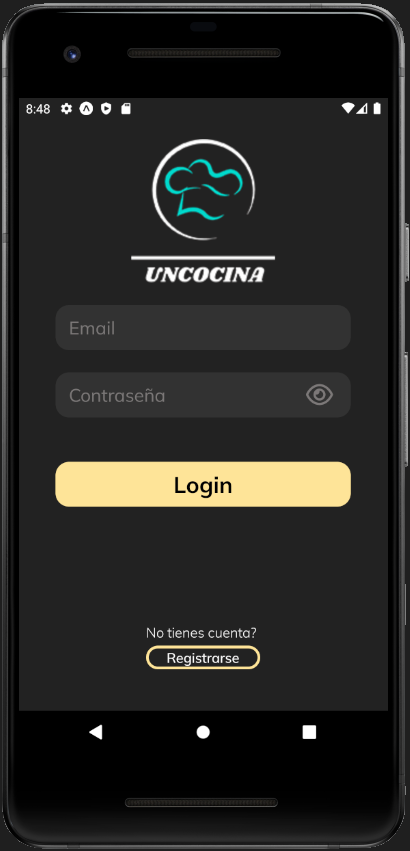
\includegraphics[width=8cm, scale=1]{Images/Imagenes/login1.png}
  \caption{Vista de inicio de sesión}
  \label{fig:login1}
\end{figure}

\begin{figure}[!h]
  \centering
  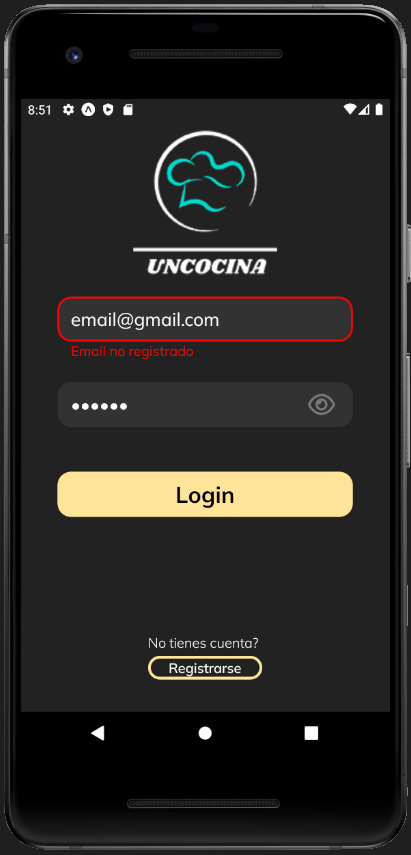
\includegraphics[width=8cm, scale=1]{Images/Imagenes/login2.png}
  \caption{Vista de inicio de sesión con validación}
  \label{fig:login2}
\end{figure}

\textbf{Vista de registro: }
Permite el registro de usuarios a la plataforma. Realiza el mismo tipo de validaciones que la pantalla de inicio de sesión. Figura \ref{fig:registro}\\

\begin{figure}[!h]
  \centering
  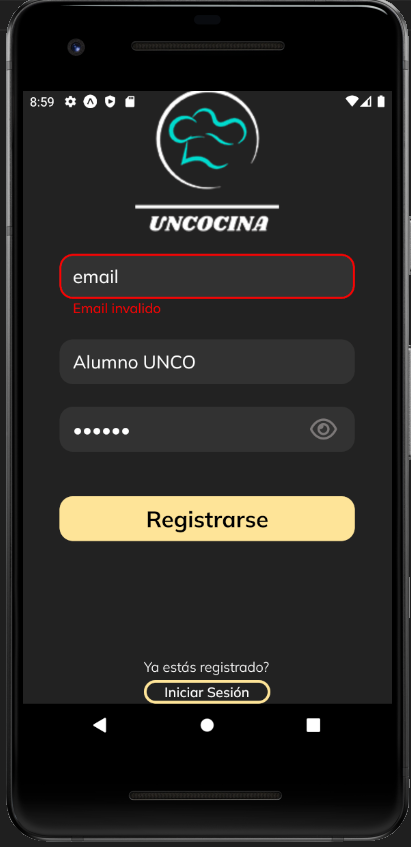
\includegraphics[width=8cm, scale=1]{Images/Imagenes/registro.png}
  \caption{Vista de registro}
  \label{fig:registro}
\end{figure}

\textbf{Vista de recetas: }
Una vez el usuario se registra o inicia sesión es redireccionado automáticamente a esta vista, aquí se mostrara todas las recetas de la base de datos permitiendo ordenarlas por fecha de publicación y filtrar por categorías. Ademas como la API soporta paginación las recetas se van cargando a medida que se ``scrollea'' hacia abajo. Figura \ref{fig:recetas1}, Figura \ref{fig:recetas2} y Figura \ref{fig:recetas3}\\

\begin{figure}[!h]
  \centering
  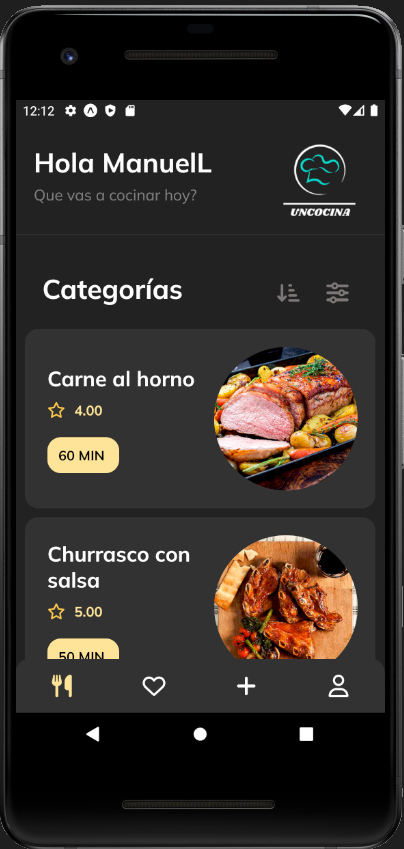
\includegraphics[width=8cm, scale=1]{Images/Imagenes/recetas1.png}
  \caption{Vista de recetas}
  \label{fig:recetas1}
\end{figure}

\begin{figure}[!h]
  \centering
  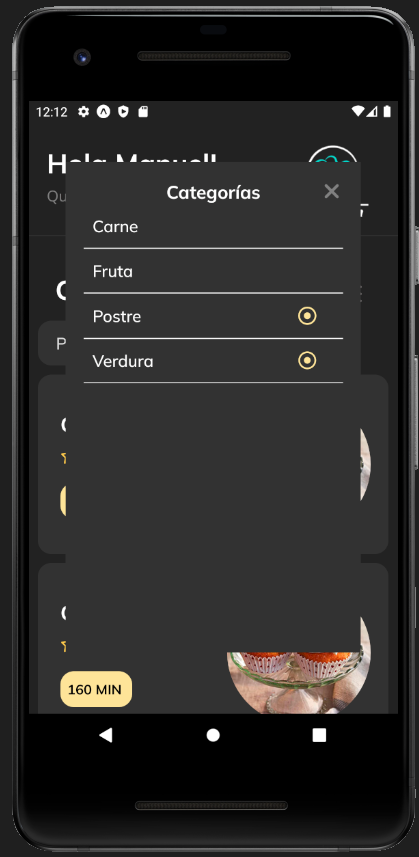
\includegraphics[width=8cm, scale=1]{Images/Imagenes/recetas2.png}
  \caption{Selección de categorías para filtrar}
  \label{fig:recetas2}
\end{figure}

\begin{figure}[!h]
  \centering
  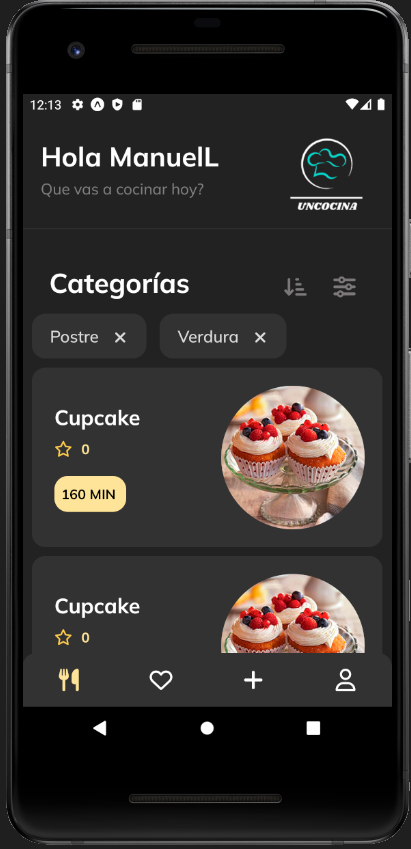
\includegraphics[width=8cm, scale=1]{Images/Imagenes/recetas3.png}
  \caption{Vista de recetas con categorías filtradas}
  \label{fig:recetas3}
\end{figure}

\textbf{Vista de favoritos: }
Esta vista reutiliza el componente utilizado para la vista de recetas para mostrar las recetas seleccionadas como favoritas por los usuarios. Puede accederse a traves del navbar ubicado en la parte baja de la pantalla. Figura \ref{fig:favoritos} y Figura \ref{fig:favoritos2}\\

\begin{figure}[!h]
  \centering
  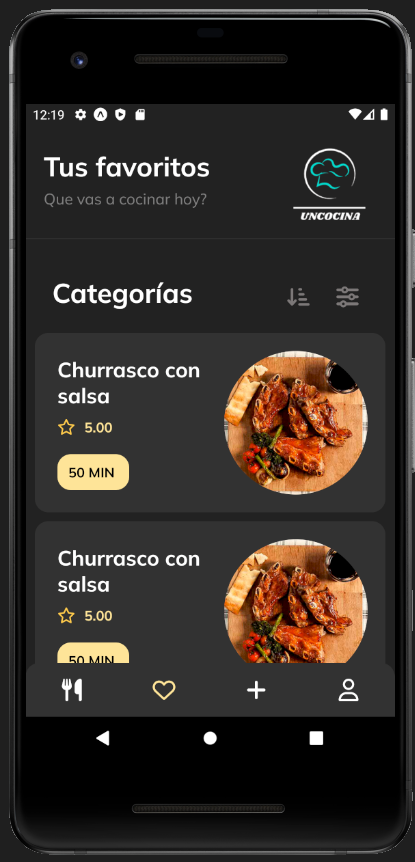
\includegraphics[width=8cm, scale=1]{Images/Imagenes/favoritos.png}
  \caption{Vista de favoritos}
  \label{fig:favoritos}
\end{figure}

\begin{figure}[!h]
  \centering
  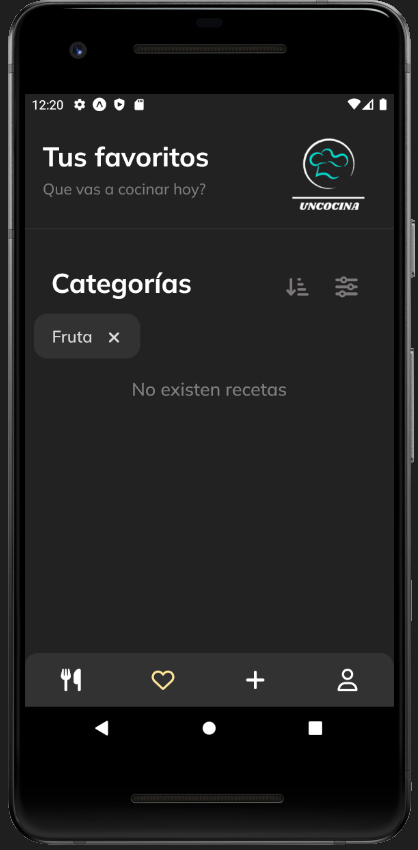
\includegraphics[width=8cm, scale=1]{Images/Imagenes/favoritos2.png}
  \caption{Vista de favoritos con una categoría de recetas seleccionada para la cual aun no existen favoritos}
  \label{fig:favoritos2}
\end{figure}

\textbf{Vista información de receta: }
Si en las vistas de recetas o favoritos se presiona sobre alguna de las recetas se llegara a la vista de información de dicha receta. Aquí se pueden ver listados los pasos de la receta, ingredientes, duración, imagen, se puede realizar una calificación sobre la receta y agregarla a favoritos. Ademas se utilizo el componente externo ``\texttt{@gorhom/bottom-sheet}'' para poner los ingredientes en un cajon deslizable. Figura \ref{fig:inforeceta1}, Figura \ref{fig:inforeceta2}, Figura \ref{fig:inforeceta3} y Figura \ref{fig:inforeceta4}\\

\begin{figure}[!h]
  \centering
  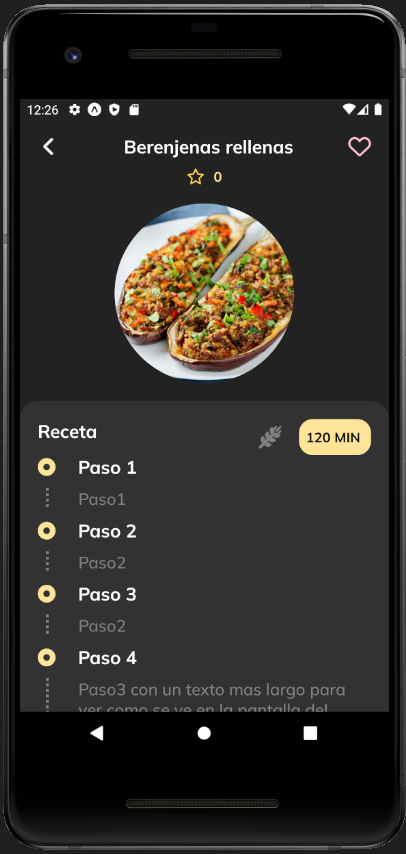
\includegraphics[width=8cm, scale=1]{Images/Imagenes/inforeceta1.png}
  \caption{Vista de información de receta}
  \label{fig:inforeceta1}
\end{figure}

\begin{figure}[!h]
  \centering
  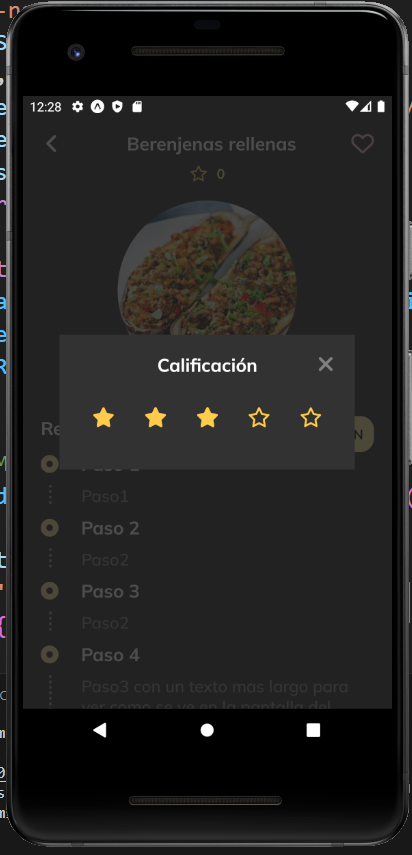
\includegraphics[width=8cm, scale=1]{Images/Imagenes/inforeceta2.png}
  \caption{Vista de calificación de receta}
  \label{fig:inforeceta2}
\end{figure}

\begin{figure}[!h]
  \centering
  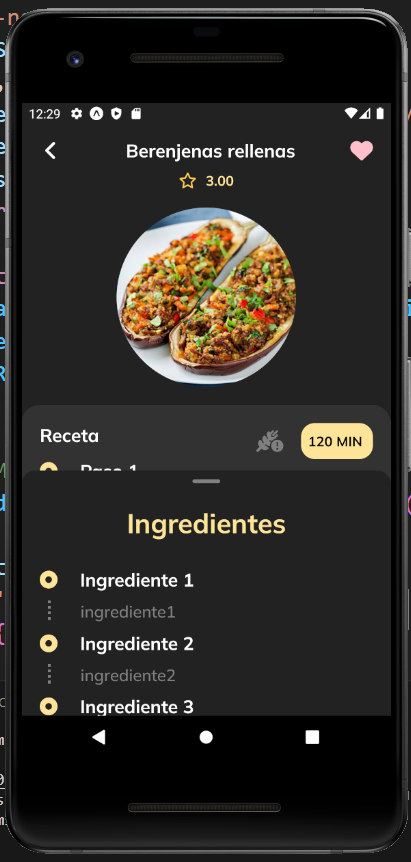
\includegraphics[width=8cm, scale=1]{Images/Imagenes/inforeceta3.png}
  \caption{Vista de información de receta con cajon de ingredientes a mitad de pantalla}
  \label{fig:inforeceta3}
\end{figure}

\begin{figure}[!h]
  \centering
  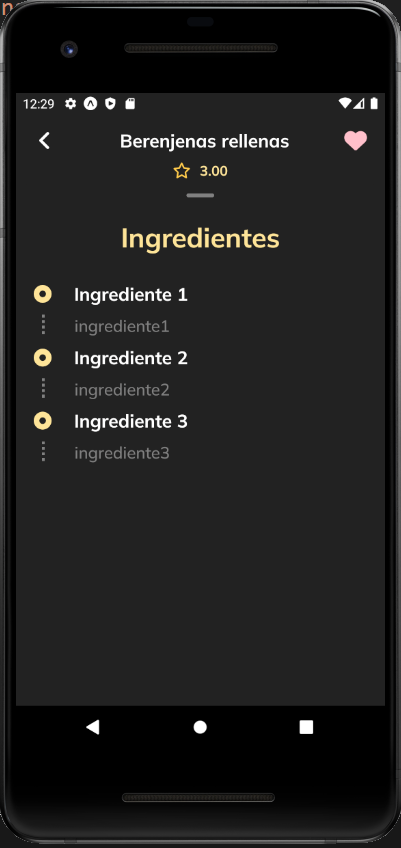
\includegraphics[width=8cm, scale=1]{Images/Imagenes/inforeceta4.png}
  \caption{Vista de calificación información de receta con cajon de ingredientes completamente abierto}
  \label{fig:inforeceta4}
\end{figure}

\textbf{Vista de creación de receta: }
En esta vista se solicitaran todos los datos necesarios para crear una nueva receta. Se realizaran las validaciones correspondientes y una vez cargada la receta exitosamente ser redireccionara a la vista de recetas donde se podrá ver publicada. Figuras [\ref{fig:add1}],[\ref{fig:add2}],[\ref{fig:add3}],[\ref{fig:add4}],[\ref{fig:add5}],[\ref{fig:add6}],[\ref{fig:add7}],[\ref{fig:add8}],[\ref{fig:add9}]\\

\begin{figure}[!h]
  \centering
  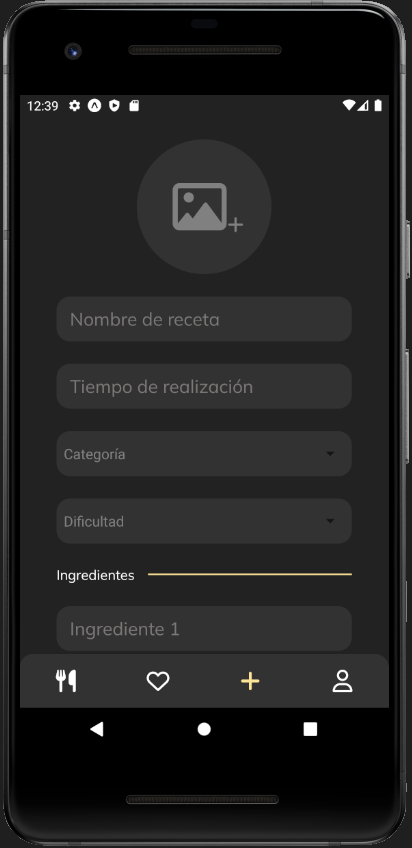
\includegraphics[width=8cm, scale=1]{Images/Imagenes/add1.png}
  \caption{Vista de creación de receta}
  \label{fig:add1}
\end{figure}

\begin{figure}[!h]
  \centering
  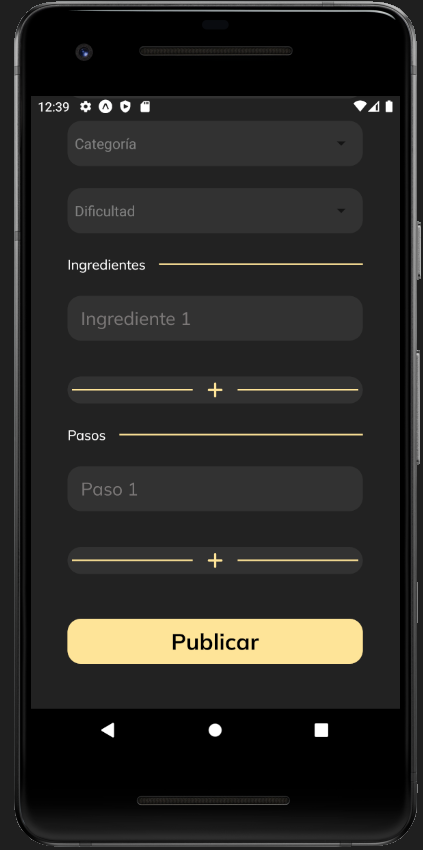
\includegraphics[width=8cm, scale=1]{Images/Imagenes/add2.png}
  \caption{Vista de creación de receta}
  \label{fig:add2}
\end{figure}

\begin{figure}[!h]
  \centering
  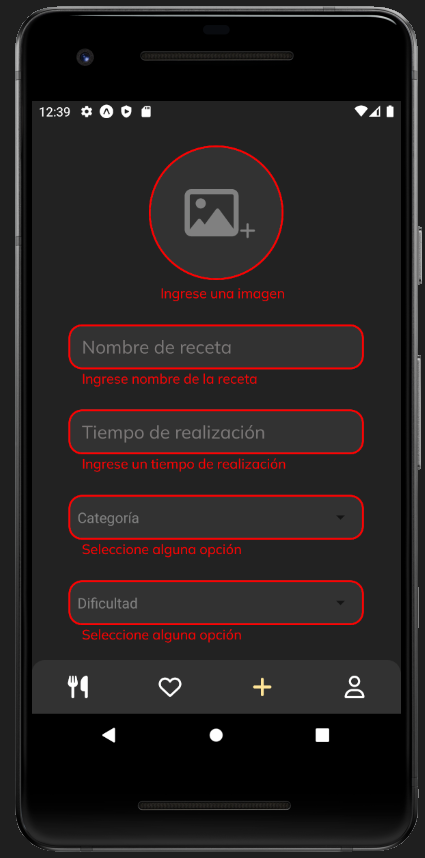
\includegraphics[width=8cm, scale=1]{Images/Imagenes/add3.png}
  \caption{Vista de creación de receta con validaciones}
  \label{fig:add3}
\end{figure}

\begin{figure}[!h]
  \centering
  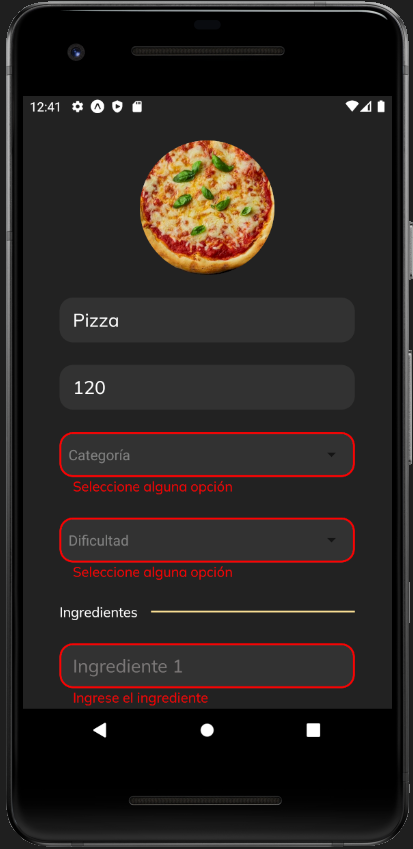
\includegraphics[width=8cm, scale=1]{Images/Imagenes/add4.png}
  \caption{Vista de creación de receta}
  \label{fig:add4}
\end{figure}

\begin{figure}[!h]
  \centering
  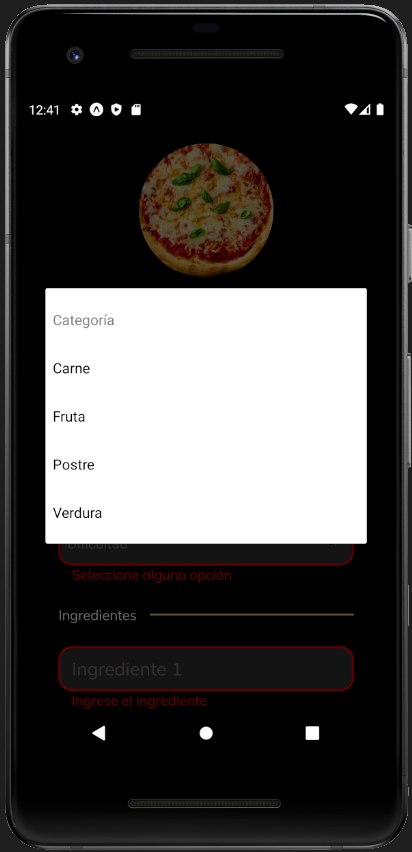
\includegraphics[width=8cm, scale=1]{Images/Imagenes/add5.png}
  \caption{Vista de creación de receta seleccionando la categoría}
  \label{fig:add5}
\end{figure}

\begin{figure}[!h]
  \centering
  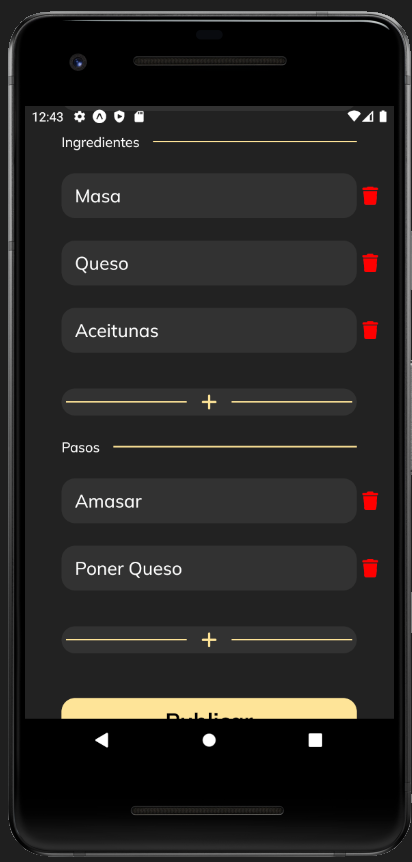
\includegraphics[width=8cm, scale=1]{Images/Imagenes/add6.png}
  \caption{Vista de creación de receta definiendo los ingredientes y pasos a seguir}
  \label{fig:add6}
\end{figure}

\begin{figure}[!h]
  \centering
  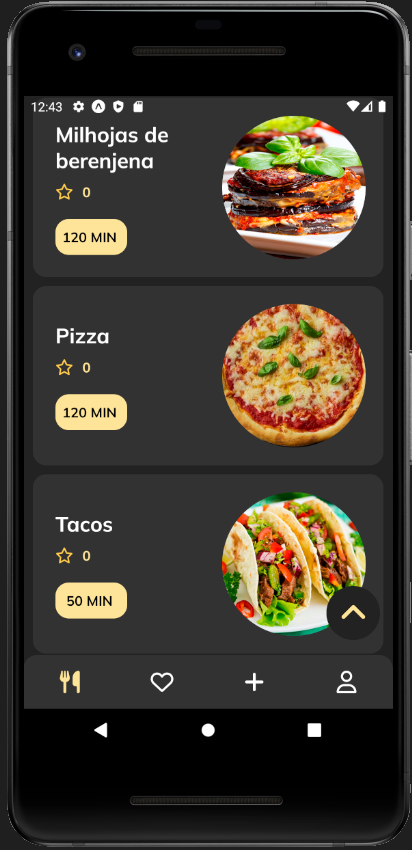
\includegraphics[width=8cm, scale=1]{Images/Imagenes/add7.png}
  \caption{Vista recetas en donde se ve la nueva receta agregada}
  \label{fig:add7}
\end{figure}

\begin{figure}[!h]
  \centering
  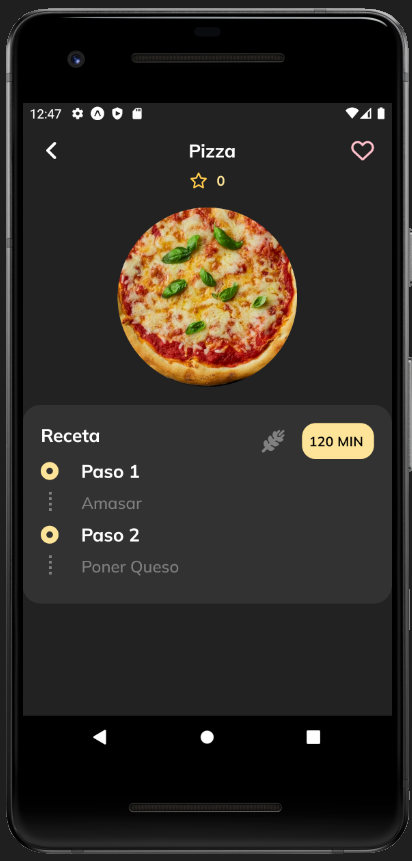
\includegraphics[width=8cm, scale=1]{Images/Imagenes/add8.png}
  \caption{Vista información de la receta creada}
  \label{fig:add8}
\end{figure}

\begin{figure}[!h]
  \centering
  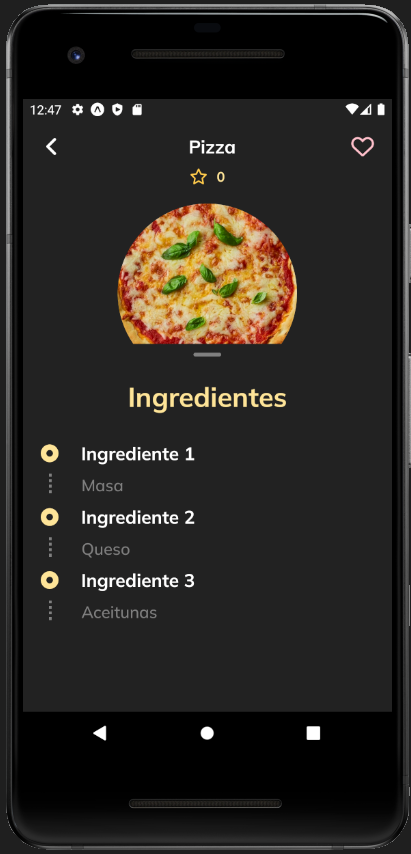
\includegraphics[width=8cm, scale=1]{Images/Imagenes/add9.png}
  \caption{Vista información de la receta creada}
  \label{fig:add9}
\end{figure}

\textbf{Vista de cierre de sesión: }
Finalmente se cuenta con una vista para cerrar la sesión, al hacerlo redirecciona automáticamente a la vista de inicio de sesión. Figura \ref{fig:cierre}

\begin{figure}[!h]
  \centering
  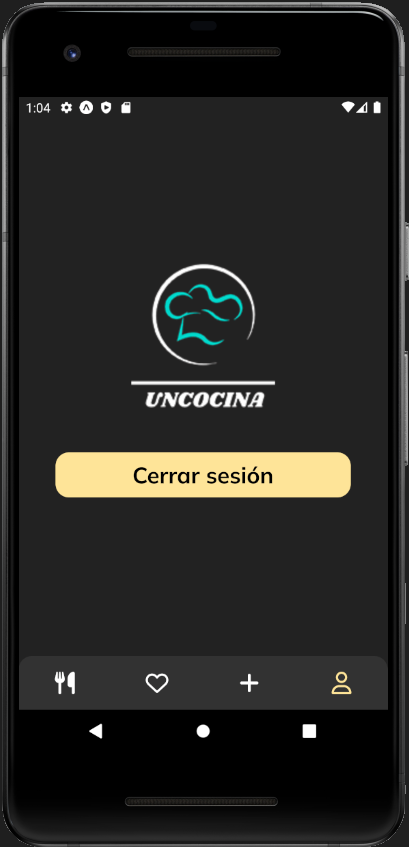
\includegraphics[width=8cm, scale=1]{Images/Imagenes/cierre.png}
  \caption{Vista cierre de sesión}
  \label{fig:cierre}
\end{figure}